% ==============================
% 正文内容（维氏硬度实验报告）
% ==============================

\begin{reportabstract}
    本实验采用维氏硬度计对标准硬度块进行硬度测试。通过施加 1~kgf 载荷，测量压痕对角线长度，计算维氏硬度值。
    实验结果表明，所测标准硬度块的维氏硬度值为 423.6~HV。
    通过本实验，掌握了显微维氏硬度计的操作方法和数据处理流程，加深了对硬度测试原理的理解。
\end{reportabstract}

% ==============================
% 一、实验原理
% ==============================

\section{实验原理}

硬度是材料抵抗局部塑性变形的能力，是衡量材料力学性能的重要指标之一。
维氏硬度（Vickers Hardness）试验由 Robert L. Smith 和 George E. Sandland 于 1921 年在 Vickers 公司提出，
因其适用范围广（从极软到极硬材料）、压痕小、精度高等优点，在材料科学与工程领域得到广泛应用。

维氏硬度试验采用面夹角为 $136^{\circ}$ 的正四棱锥金刚石压头，
在规定载荷 $F$ 作用下压入试样表面，保持规定时间后卸除载荷，
测量压痕对角线长度 $d_1$、$d_2$，取平均值 $d = (d_1 + d_2)/2$。

维氏硬度值（HV）定义为载荷与压痕表面积之比：
\begin{equation}
    HV = \frac{2F \sin(136^{\circ}/2)}{d^2} \approx 1.8544 \frac{F}{d^2}
\end{equation}
其中 $F$ 单位为 kgf，$d$ 单位为 mm。

% ==============================
% 二、实验方案
% ==============================

\section{实验方案}

\subsection{实验设备与材料}

\begin{itemize}
    \item 显微维氏硬度计（型号：HV-1000 型）
    \item 标准硬度块
    \item 测量显微镜
    \item 金相抛光设备
\end{itemize}

\subsection{实验参数设计}

\begin{itemize}
    \item 试验载荷：$F = 1$~kgf（约 9.8 N）
    \item 保载时间：10 秒
    \item 测试点数：在试样表面选取多个不同位置进行测试
    \item 测量内容：压痕两条对角线长度 $d_1$、$d_2$，计算平均值 $d$ 及 HV 值
\end{itemize}

% ==============================
% 三、实验过程
% ==============================

\section{实验过程}

\begin{enumerate}[label=\arabic*., leftmargin=2em]
    \item \textbf{试样准备}：对待测试样进行打磨、抛光处理，确保表面平整光洁，无氧化层和划痕；
    \item \textbf{设备校准}：使用标准硬度块对维氏硬度计进行校准，确保测量精度；
    \item \textbf{选择载荷}：根据材料类型选择试验载荷为 1~kgf，设置保载时间；
    \item \textbf{加载测试}：将试样置于载物台，调整焦距使表面清晰成像，施加选定载荷并保持 10 秒；
    \item \textbf{测量压痕}：卸除载荷后，用测量显微镜读取压痕两条对角线长度 $d_1$、$d_2$，取平均值；
    \item \textbf{重复测试}：在试样不同位置重复上述步骤，记录多组数据以保证结果可靠性；
    \item \textbf{显微观察}：拍摄压痕显微照片，观察压痕形貌。
\end{enumerate}

\begin{figure}[htbp]
    \centering
    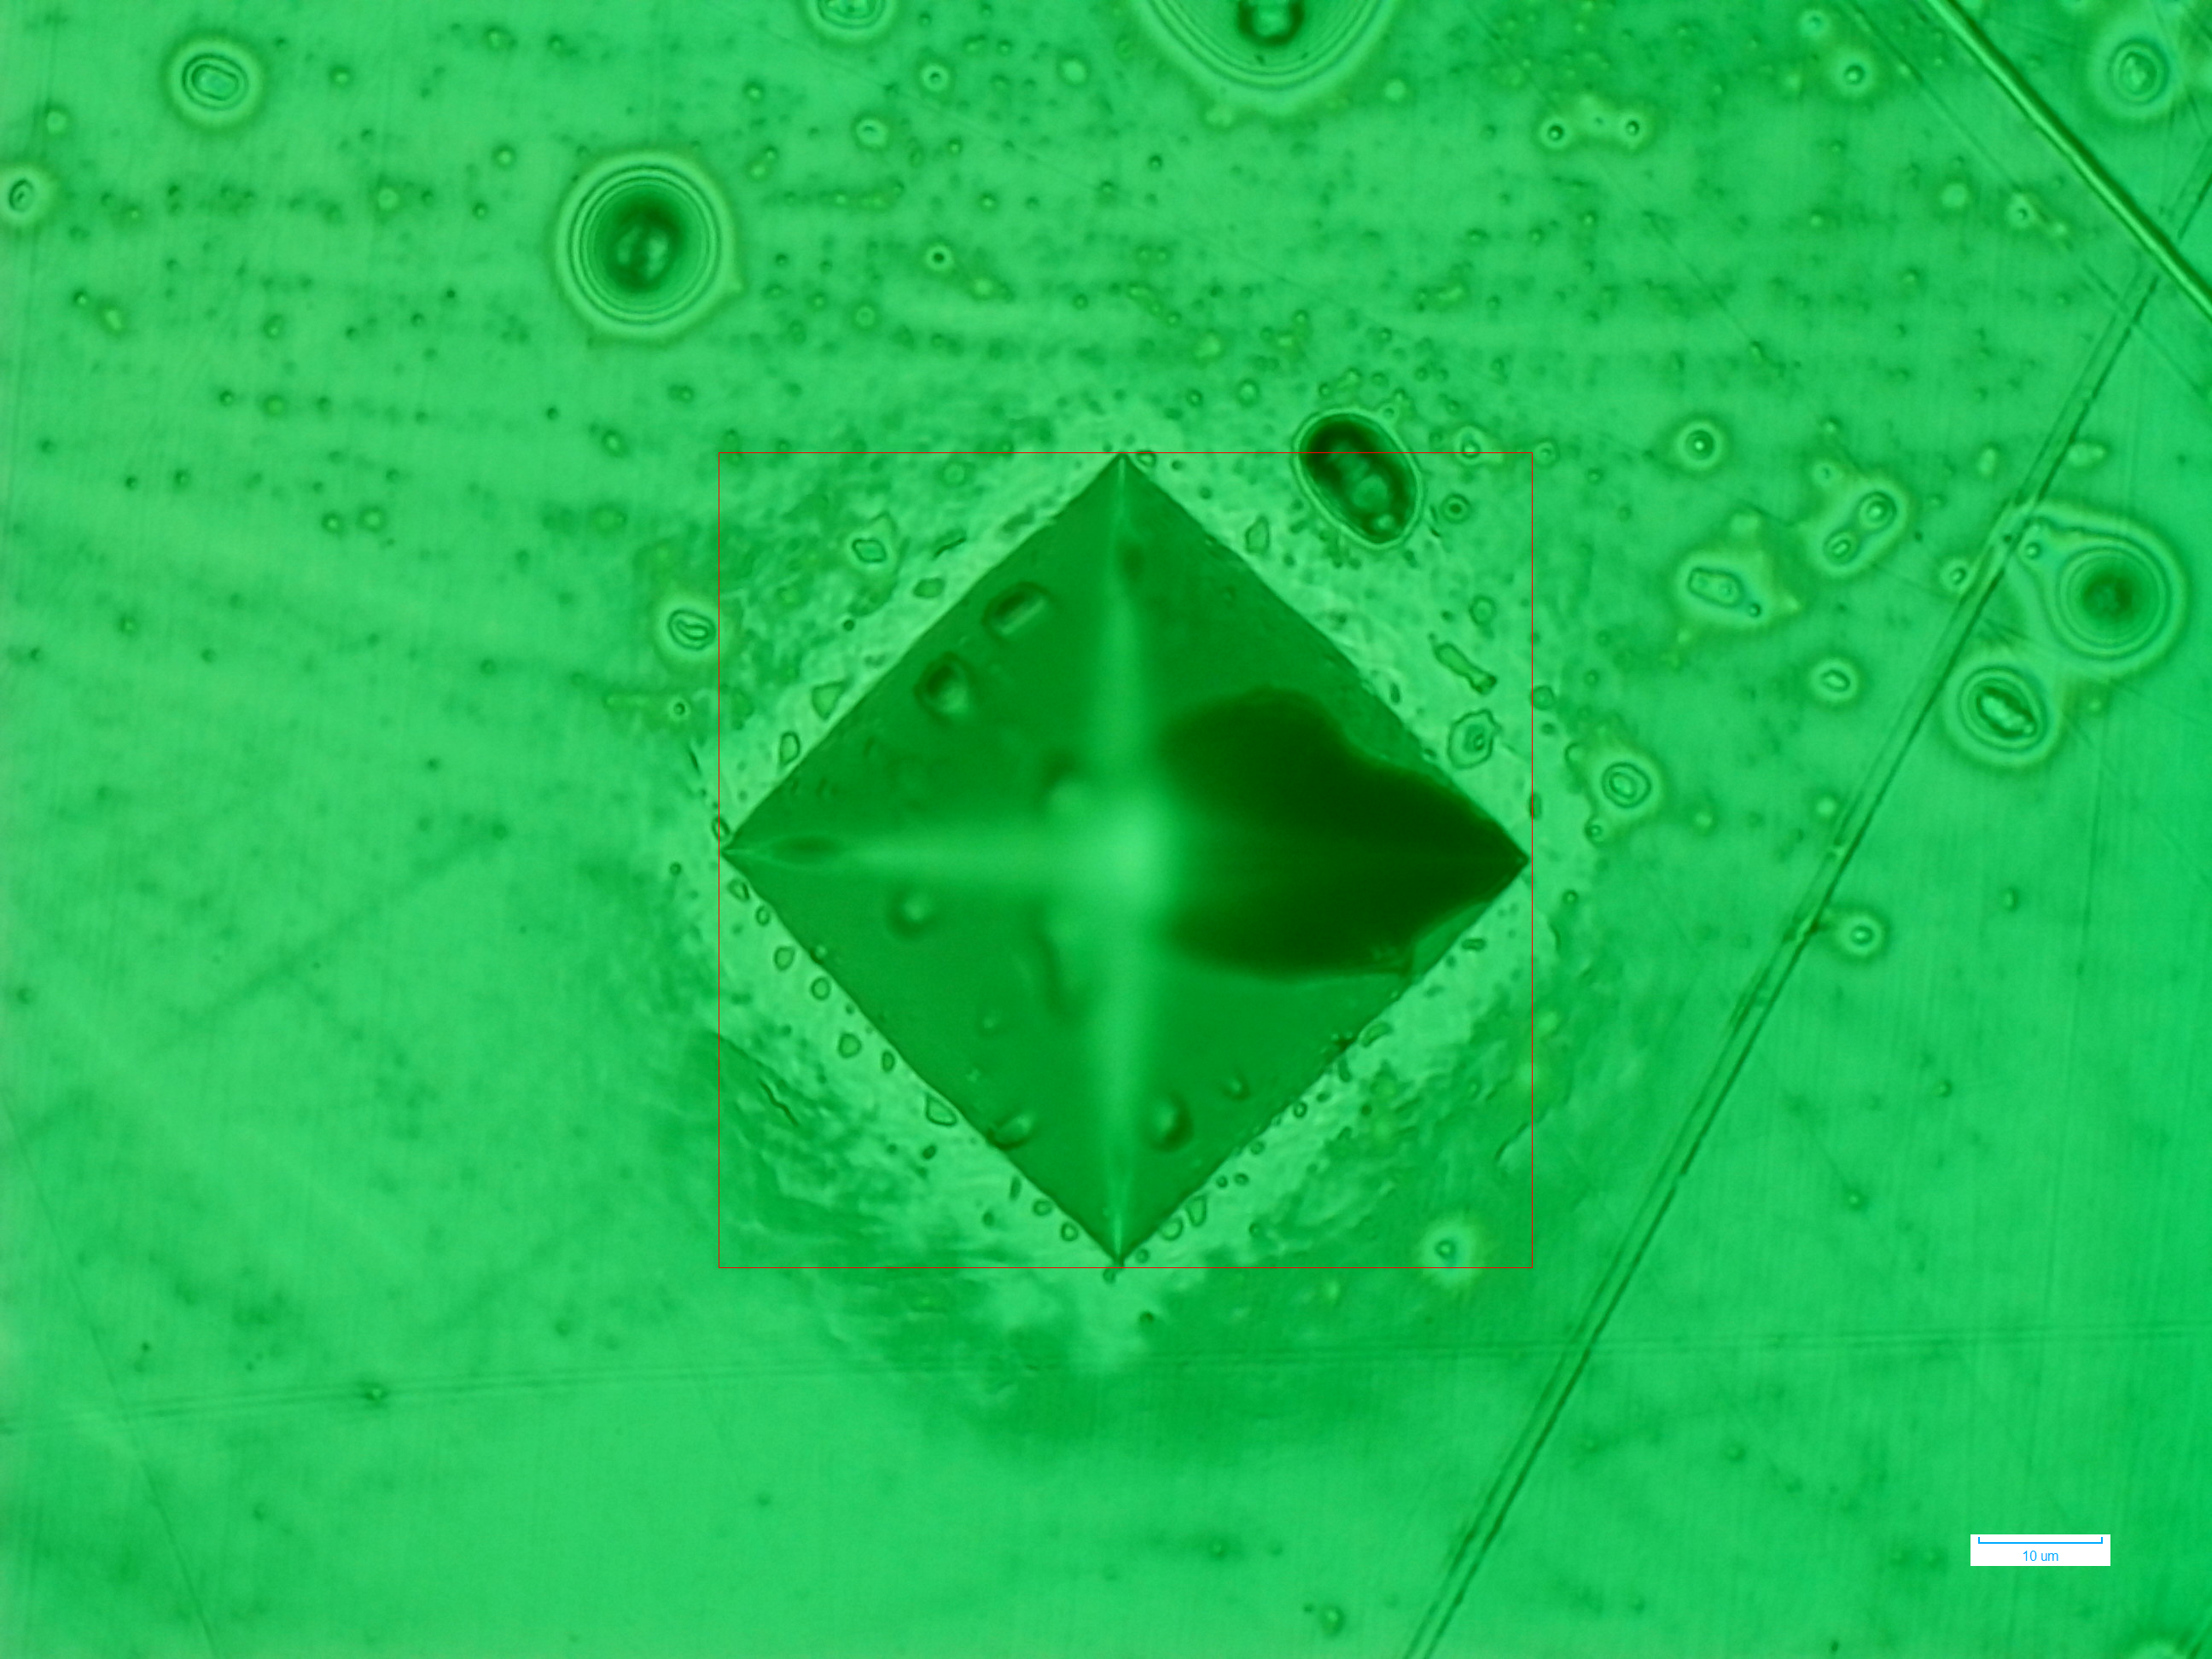
\includegraphics[width=0.55\textwidth]{../data/output.files/压痕图.png}
    \caption{维氏硬度压痕显微形貌（载荷 1~kgf）}
    \label{fig:indentation}
\end{figure}

如图~\ref{fig:indentation} 所示，压痕呈规整的正四棱锥形状，两条对角线清晰可辨，表明试样表面制备质量良好，测试结果可靠。

% ==============================
% 四、数据分析
% ==============================

\section{数据分析}

\subsection{实验数据记录}

本次实验采用载荷 $F = 1$~kgf（即 1000~g），在试样表面选取测试点进行维氏硬度测试。
实验数据如表~\ref{tab:hardness} 所示。

\begin{table}[htbp]
    \centering
    \caption{维氏硬度测试数据（$F = 1$~kgf）}
    \label{tab:hardness}
    \begin{tabular}{cccccc}
        \toprule
        测量点 & $d_1$ (\textmu m) & $d_2$ (\textmu m) & $d$ (\textmu m) & $F$ (kgf) & HV \\
        \midrule
        1 & 66.1 & 66.2 & 66.15 & 1 & 423.6 \\
        \bottomrule
    \end{tabular}
\end{table}

\subsection{硬度值计算}

平均对角线长度：
\begin{equation}
    d = \frac{d_1 + d_2}{2} = \frac{66.1 + 66.2}{2} = 66.15\;\mu\text{m} = 0.06615\;\text{mm}
\end{equation}

维氏硬度值按公式计算：
\begin{equation}
    HV = 1.8544 \times \frac{F}{d^2} = 1.8544 \times \frac{1}{(0.06615)^2} \approx 423.8\;\text{HV}
\end{equation}

与仪器直接读数值 423.6~HV 基本一致，差异来源于四舍五入误差。

\begin{figure}[htbp]
    \centering
    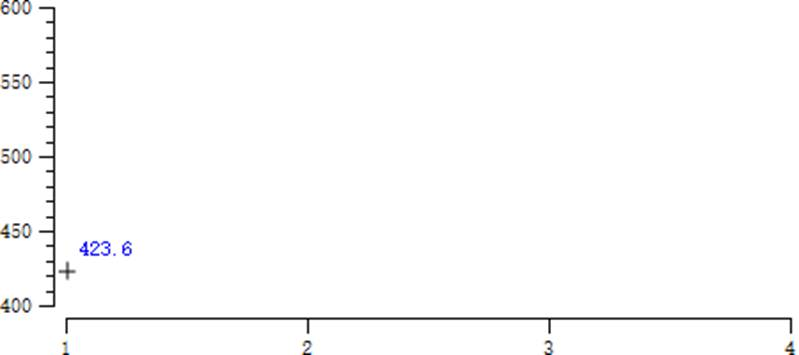
\includegraphics[width=0.75\textwidth]{../data/output.files/硬化曲线.jpg}
    \caption{维氏硬度测试结果曲线}
    \label{fig:hardness-curve}
\end{figure}

如图~\ref{fig:hardness-curve} 所示，硬度测试结果曲线直观地展示了所测硬度值 423.6~HV 在坐标系中的位置。

\subsection{硬度值分析与讨论}

\textbf{硬度值分析：} 测得维氏硬度值为 423.6~HV。由于实验样品为标准硬度块，其硬度值是经过标定的，
本次测量结果可用于验证硬度计的工作状态和测量精度。

\textbf{误差分析：} 影响维氏硬度测量精度的主要因素包括：
\begin{enumerate}[label=(\arabic*)]
    \item \textbf{试样表面质量：} 表面粗糙度会导致压痕边缘模糊，影响对角线测量精度；
    \item \textbf{载荷选择：} 载荷过小，压痕尺寸小，测量相对误差增大；载荷过大，可能导致试样变形或裂纹；
    \item \textbf{压痕测量误差：} 显微镜读数精度及操作者主观判断引入的误差；
    \item \textbf{设备因素：} 硬度计加载系统的精度、压头几何形状的偏差等；
    \item \textbf{材料不均匀性：} 材料微观组织的不均匀可能导致不同位置硬度值存在差异。
\end{enumerate}

建议在后续实验中增加测量点数（至少 5 点），并进行统计分析（计算平均值、标准差和变异系数），
以更全面地评估材料的硬度特性。

% ==============================
% 五、实验结论
% ==============================

\section{实验结论}

通过本次维氏硬度实验，得出以下结论：

\begin{enumerate}[label=(\arabic*)]
    \item 所测标准硬度块的维氏硬度约为 423.6~HV（载荷 1~kgf）；
    \item 实验结果表明维氏硬度测试具有操作简便、结果可靠的特点；
    \item 掌握了维氏硬度计的操作方法和数据处理流程；
    \item 理解了载荷、压痕对角线长度与硬度值之间的定量关系；
    \item 学会了标准硬度块的使用和保养方法，了解了硬度计校准的基本流程。
\end{enumerate}

% ==============================
% 六、心得体会
% ==============================

\section{心得体会}

通过本次维氏硬度实验，我对材料硬度测试有了更加深入的理解和体会：

\begin{enumerate}[label=(\arabic*)]
    \item 维氏硬度试验虽然原理简单，但实际操作中需要注意细节：试样表面的制备质量直接影响压痕的清晰度和测量精度，抛光的均匀性尤为关键；
    \item 压痕对角线的测量是误差的主要来源之一。实验中需要耐心、细致地调节显微镜焦距，多次读取取平均值，以减小人为误差；
    \item 通过亲手操作硬度计和数据处理，加深了对 $HV = 1.8544F/d^2$ 公式物理意义的理解，体会到了理论推导与工程应用的紧密结合；
    \item 了解了标准硬度块在硬度计校准中的重要作用——硬度块具有已知的标准硬度值，可用来验证仪器的测量准确性和重复性；
    \item 本次实验培养了我严谨的科学态度和数据分析能力，为今后的材料科学实验和研究工作打下了良好基础。
\end{enumerate}